
\documentclass[letterpaper,hide notes,xcolor={table,svgnames},pdftex,10pt]{beamer}
\def\showexamples{t}


%\usepackage[svgnames]{xcolor}

%% Demo talk
%\documentclass[letterpaper,notes=show]{beamer}

\usecolortheme{crane}
\setbeamertemplate{navigation symbols}{}

\usetheme{MyPittsburgh}
%\usetheme{Frankfurt}

%\usepackage{tipa}

\usepackage{hyperref}
\usepackage{graphicx,xspace}
\usepackage[normalem]{ulem}
\usepackage{multicol}
\usepackage{amsmath,amssymb,amsthm,graphicx,xspace}
\newcommand\SF[1]{$\bigstar$\footnote{SF: #1}}

\usepackage[default]{sourcesanspro}
\usepackage[T1]{fontenc}
\usepackage[scaled]{beramono}
\usepackage{tikzpagenodes}

\newcounter{tmpnumSlide}
\newcounter{tmpnumNote}


% old question code
%\newcommand\question[1]{{$\bigstar$ \small \onlySlide{2}{#1}}}
% \newcommand\nquestion[1]{\ifdefined \presentationonly \textcircled{?} \fi \note{\par{\Large \textbf{?}} #1}}
% \newcommand\nanswer[1]{\note{\par{\Large \textbf{A}} #1}}


 \newcommand\mnote[1]{%
   \addtocounter{tmpnumSlide}{1}
   \ifdefined\showcues {~\tiny\fbox{\arabic{tmpnumSlide}}}\fi
   \note{\setlength{\parskip}{1ex}\addtocounter{tmpnumNote}{1}\textbf{\Large \arabic{tmpnumNote}:} {#1\par}}}

\newcommand\mmnote[1]{\note{\setlength{\parskip}{1ex}#1\par}}

%\newcommand\mnote[2][]{\ifdefined\handoutwithnotes {~\tiny\fbox{#1}}\fi
% \note{\setlength{\parskip}{1ex}\textbf{\Large #1:} #2\par}}

%\newcommand\mnote[2][]{{\tiny\fbox{#1}} \note{\setlength{\parskip}{1ex}\textbf{\Large #1:} #2\par}}

\newcommand\mquestion[2]{{~\color{red}\fbox{?}}\note{\setlength{\parskip}{1ex}\par{\Large \textbf{?}} #1} \note{\setlength{\parskip}{1ex}\par{\Large \textbf{A}} #2\par}\ifdefined \presentationonly \pause \fi}

\newcommand\blackboard[1]{%
\ifdefined   \showblackboard
  {#1}
  \else {\begin{center} \fbox{\colorbox{blue!30}{%
         \begin{minipage}{.95\linewidth}%
           \hspace{\stretch{1}} Some space intentionally left blank; done at the blackboard.%
         \end{minipage}}}\end{center}}%
         \fi%
}



%\newcommand\q{\tikz \node[thick,color=black,shape=circle]{?};}
%\newcommand\q{\ifdefined \presentationonly \textcircled{?} \fi}

\usepackage{listings}
\lstset{basicstyle=\footnotesize\ttfamily,
	breaklines=true,
	aboveskip=15pt,
  	belowskip=15pt,
	frame=lines,
	numbers=left, basicstyle=\scriptsize, numberstyle=\tiny, stepnumber=0, numbersep=2pt
}

\usepackage{siunitx}
\newcommand\sius[1]{\num[group-separator = {,}]{#1}\si{\micro\second}}
\newcommand\sims[1]{\num[group-separator = {,}]{#1}\si{\milli\second}}
\newcommand\sins[1]{\num[group-separator = {,}]{#1}\si{\nano\second}}
\sisetup{group-separator = {,}, group-digits = true}

%% -------------------- tikz --------------------
\usepackage{tikz}
\usetikzlibrary{positioning}
\usetikzlibrary{arrows,backgrounds,automata,decorations.shapes,decorations.pathmorphing,decorations.markings,decorations.text,decorations.pathreplacing}

\tikzstyle{place}=[circle,draw=blue!50,fill=blue!20,thick, inner sep=0pt,minimum size=6mm]
\tikzstyle{transition}=[rectangle,draw=black!50,fill=black!20,thick, inner sep=0pt,minimum size=4mm]

\tikzstyle{block}=[rectangle,draw=black, thick, inner sep=5pt]
\tikzstyle{bullet}=[circle,draw=black, fill=black, thin, inner sep=2pt]

\tikzstyle{pre}=[<-,shorten <=1pt,>=stealth',semithick]
\tikzstyle{post}=[->,shorten >=1pt,>=stealth',semithick]
\tikzstyle{bi}=[<->,shorten >=1pt,shorten <=1pt, >=stealth',semithick]

\tikzstyle{mut}=[-,>=stealth',semithick]

\tikzstyle{treereset}=[dashed,->, shorten >=1pt,>=stealth',thin]

\usepackage{ifmtarg}
\usepackage{xifthen}
\makeatletter
% new counter to now which frame it is within the sequence
\newcounter{multiframecounter}
% initialize buffer for previously used frame title
\gdef\lastframetitle{\textit{undefined}}
% new environment for a multi-frame
\newenvironment{multiframe}[1][]{%
\ifthenelse{\isempty{#1}}{%
% if no frame title was set via optional parameter,
% only increase sequence counter by 1
\addtocounter{multiframecounter}{1}%
}{%
% new frame title has been provided, thus
% reset sequence counter to 1 and buffer frame title for later use
\setcounter{multiframecounter}{1}%
\gdef\lastframetitle{#1}%
}%
% start conventional frame environment and
% automatically set frame title followed by sequence counter
\begin{frame}%
\frametitle{\lastframetitle~{\normalfont(\arabic{multiframecounter})}}%
}{%
\end{frame}%
}
\makeatother

\makeatletter
\newdimen\tu@tmpa%
\newdimen\ydiffl%
\newdimen\xdiffl%
\newcommand\ydiff[2]{%
    \coordinate (tmpnamea) at (#1);%
    \coordinate (tmpnameb) at (#2);%
    \pgfextracty{\tu@tmpa}{\pgfpointanchor{tmpnamea}{center}}%
    \pgfextracty{\ydiffl}{\pgfpointanchor{tmpnameb}{center}}%
    \advance\ydiffl by -\tu@tmpa%
}
\newcommand\xdiff[2]{%
    \coordinate (tmpnamea) at (#1);%
    \coordinate (tmpnameb) at (#2);%
    \pgfextractx{\tu@tmpa}{\pgfpointanchor{tmpnamea}{center}}%
    \pgfextractx{\xdiffl}{\pgfpointanchor{tmpnameb}{center}}%
    \advance\xdiffl by -\tu@tmpa%
}
\makeatother
\newcommand{\copyrightbox}[3][r]{%
\begin{tikzpicture}%
\node[inner sep=0pt,minimum size=2em](ciimage){#2};
\usefont{OT1}{phv}{n}{n}\fontsize{4}{4}\selectfont
\ydiff{ciimage.south}{ciimage.north}
\xdiff{ciimage.west}{ciimage.east}
\ifthenelse{\equal{#1}{r}}{%
\node[inner sep=0pt,right=1ex of ciimage.south east,anchor=north west,rotate=90]%
{\raggedleft\color{black!50}\parbox{\the\ydiffl}{\raggedright{}#3}};%
}{%
\ifthenelse{\equal{#1}{l}}{%
\node[inner sep=0pt,right=1ex of ciimage.south west,anchor=south west,rotate=90]%
{\raggedleft\color{black!50}\parbox{\the\ydiffl}{\raggedright{}#3}};%
}{%
\node[inner sep=0pt,below=1ex of ciimage.south west,anchor=north west]%
{\raggedleft\color{black!50}\parbox{\the\xdiffl}{\raggedright{}#3}};%
}
}
\end{tikzpicture}
}


%% --------------------

%\usepackage[excludeor]{everyhook}
%\PushPreHook{par}{\setbox0=\lastbox\llap{MUH}}\box0}

%\vspace*{\stretch{1}

%\setbox0=\lastbox \llap{\textbullet\enskip}\box0}

\setlength{\parskip}{\fill}

\newcommand\noskips{\setlength{\parskip}{1ex}}
\newcommand\doskips{\setlength{\parskip}{\fill}}

\newcommand\xx{\par\vspace*{\stretch{1}}\par}
\newcommand\xxs{\par\vspace*{2ex}\par}
\newcommand\tuple[1]{\langle #1 \rangle}
\newcommand\code[1]{{\sf \footnotesize #1}}
\newcommand\ex[1]{\uline{Example:} \ifdefined \presentationonly \pause \fi
  \ifdefined\showexamples#1\xspace\else{\uline{\hspace*{2cm}}}\fi}

\newcommand\ceil[1]{\lceil #1 \rceil}


\AtBeginSection[]
{
   \begin{frame}
       \frametitle{Outline}
       \tableofcontents[currentsection]
   \end{frame}
}



\pgfdeclarelayer{edgelayer}
\pgfdeclarelayer{nodelayer}
\pgfsetlayers{edgelayer,nodelayer,main}

\tikzstyle{none}=[inner sep=0pt]
\tikzstyle{rn}=[circle,fill=Red,draw=Black,line width=0.8 pt]
\tikzstyle{gn}=[circle,fill=Lime,draw=Black,line width=0.8 pt]
\tikzstyle{yn}=[circle,fill=Yellow,draw=Black,line width=0.8 pt]
\tikzstyle{empty}=[circle,fill=White,draw=Black]
\tikzstyle{bw} = [rectangle, draw, fill=blue!20, 
    text width=4em, text centered, rounded corners, minimum height=2em]
    
    \newcommand{\CcNote}[1]{% longname
	This work is licensed under the \textit{Creative Commons #1 3.0 License}.%
}
\newcommand{\CcImageBy}[1]{%
	\includegraphics[scale=#1]{creative_commons/cc_by_30.pdf}%
}
\newcommand{\CcImageSa}[1]{%
	\includegraphics[scale=#1]{creative_commons/cc_sa_30.pdf}%
}
\newcommand{\CcImageNc}[1]{%
	\includegraphics[scale=#1]{creative_commons/cc_nc_30.pdf}%
}
\newcommand{\CcGroupBySa}[2]{% zoom, gap
	\CcImageBy{#1}\hspace*{#2}\CcImageNc{#1}\hspace*{#2}\CcImageSa{#1}%
}
\newcommand{\CcLongnameByNcSa}{Attribution-NonCommercial-ShareAlike}

\newenvironment{changemargin}[1]{% 
  \begin{list}{}{% 
    \setlength{\topsep}{0pt}% 
    \setlength{\leftmargin}{#1}% 
    \setlength{\rightmargin}{1em}
    \setlength{\listparindent}{\parindent}% 
    \setlength{\itemindent}{\parindent}% 
    \setlength{\parsep}{\parskip}% 
  }% 
  \item[]}{\end{list}} 




\title{Lecture 28 --- Profiler Guided Optimization }

\author{Jeff Zarnett \\ \small \texttt{jzarnett@uwaterloo.ca}}
\institute{Department of Electrical and Computer Engineering \\
  University of Waterloo}
\date{\today}


\begin{document}

\begin{frame}
  \titlepage

 \end{frame}

\begin{frame}
\frametitle{Profiler Guided Optimization}


The compiler does a great deal of static analysis of the code you've written and makes its best guesses about what is likely to happen. 

The canonical example for this is branch prediction. 

There is an if-else block and the compiler will then guess about which is more likely and optimize for that version. 

\end{frame}



\begin{frame}
\frametitle{Profiler Guided Optimization}


\begin{center}
	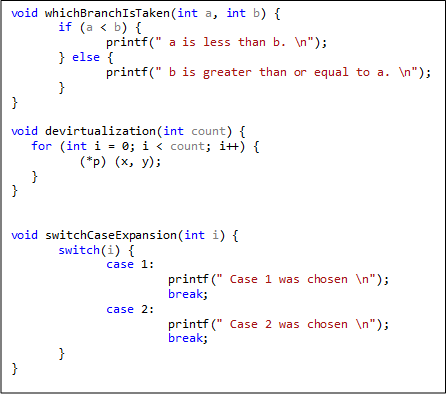
\includegraphics[width=0.65\textwidth]{images/4621codesnippet.png}
\end{center}

\end{frame}



\begin{frame}
\frametitle{Hints and Java}

There exists a solution to this, and it is that we can give hints to the compiler, but that's a manual process. 

The Java HotSpot virtual machine will update its predictions on the fly. 

There are some initial predictions and if they turn out to be wrong, the Just In Time compiler will replace it with the other version. 

The compiler runs and it does its job and that's it; the program is never updated with newer predictions if more data becomes known.

\end{frame}



\begin{frame}
\frametitle{Three Steps}

Solving this problem is the goal of POGO. 

It is taking the data from some actual runs of the program and using that to inform the predictions. 

This necessitates a multi-step compile: first compile the code, run it to collect data, then recompile the code using the data we collected.


\end{frame}



\begin{frame}
\frametitle{Step One: Measure}

Step one is to generate an executable with instrumentation. 

The compiler inserts a bunch of probes into the generated code that are used to record data. 

Three types of probe are inserted: 
\begin{itemize}
\item Function entry probes
\item Edge probes
\item Value probes
\end{itemize}

When this phase is complete, there is an instrumented executable and an empty database file where the training data goes.

\end{frame}



\begin{frame}
\frametitle{Step Two: Training Day}

\begin{center}
	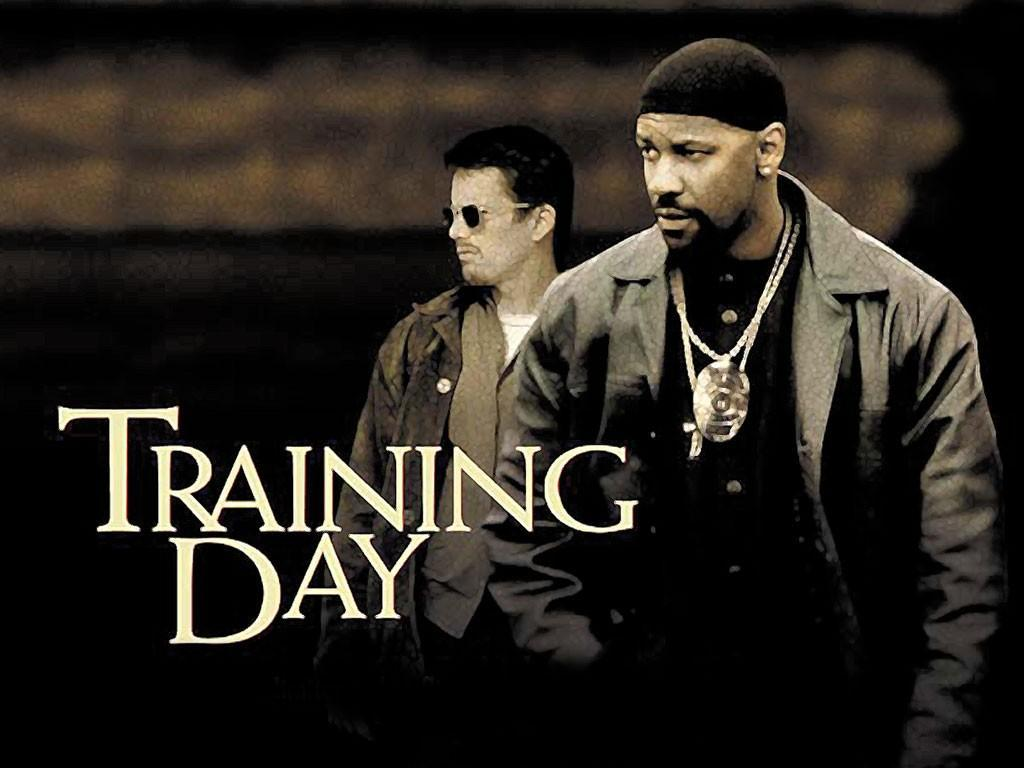
\includegraphics[width=0.6\textwidth]{images/training-day.jpg}
\end{center}

\end{frame}


\begin{frame}
\frametitle{Step Two: Training Day}

Run the instrumented executable through real-world scenarios. 

Ideally you will spend the training time on the performance-critical sections. 

It does not have to be a single training run, of course, data can be collected from as many runs as desired. 

\end{frame}



\begin{frame}
\frametitle{Step Two: Training Day}

You are not trying to exercise every part of the program (this is not unit testing)!

In fact, trying to use every bell and whistle of the program is counterproductive.

If the usage data does not match real world scenarios then  the compiler has been given the wrong information about what is important. 

Or you might end up teaching it that almost nothing is important...

\end{frame}



\begin{frame}
\frametitle{Step Three: Recompile}

Step three is a recompile. 

This time, in addition to the source files, the training data is fed into the compiler for a second compile. 

This data is applied to produce a better output executable than could be achieved by static analysis alone.

\end{frame}



\begin{frame}
\frametitle{Summary Graphic}

\begin{center}
	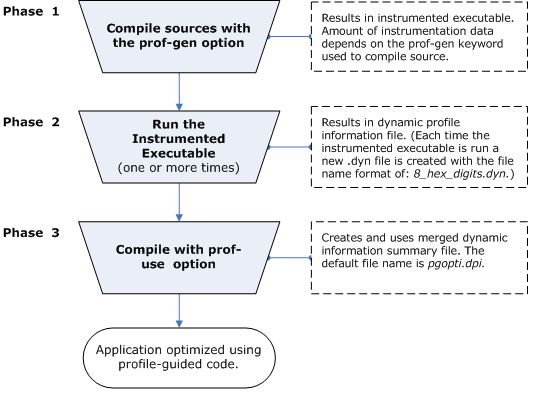
\includegraphics[width=0.75\textwidth]{images/pogo-workflow.jpg}
\end{center}

\end{frame}



\begin{frame}
\frametitle{Save Some Steps}

It is not necessary to do all three steps for every build. 

Old training data can be re-used until the code base has diverged significantly enough from the instrumented version. 

Recommended workflow: one developer performs these steps and check the training data into source control so that other developers can make use of it .

\end{frame}



\begin{frame}
\frametitle{Define ``Better''}

What does it mean for it to be better? 

The algorithms will aim for speed in the areas that are ``hot''. 

The algorithms will aim to minimize the size of code of areas that are ``cold'' .

Something less than 5\% of methods should be compiled for speed.

\end{frame}



\begin{frame}
\frametitle{Training Runs}

It is possible that we can combine multiple training runs and we can manually give some suggestions of what scenarios are important. 

Obviously the more a scenario runs in the training data, the more important it will be, as far as the POGO optimization routine is concerned. 

Multiple runs can be merged with user assigned weightings.

\end{frame}



\begin{frame}
\frametitle{Show, Don't Tell}

With the theory behind us, perhaps a demonstration about how it works is in order. 

Let us consider an example using the N-Body problem. 

Let's look at the video \url{https://www.youtube.com/watch?v=zEsdBcu4R00&t=21m45s}\\ (from 21:45 to 34:23).

\end{frame}



\begin{frame}
\frametitle{Behind the Scenes}

In the optimize phase, the training data is used to do the following optimizations:

\begin{enumerate}
\item Full and partial inlining
\item Function layout
\item Speed and size decision
\item Basic block layout 
\item Code separation
\item Virtual call speculation
\item Switch expansion
\item Data separation
\item Loop unrolling
\end{enumerate}

\end{frame}



\begin{frame}
\frametitle{Muh Gainz}

The majority of the performance gains relate to the inlining decisions. 

These decisions are based on the call graph path profiling. 

The behaviour of function \texttt{foo} may be very different when calling it from \texttt{bar} than it is when calling it from function \texttt{baz}. 


\begin{center}
	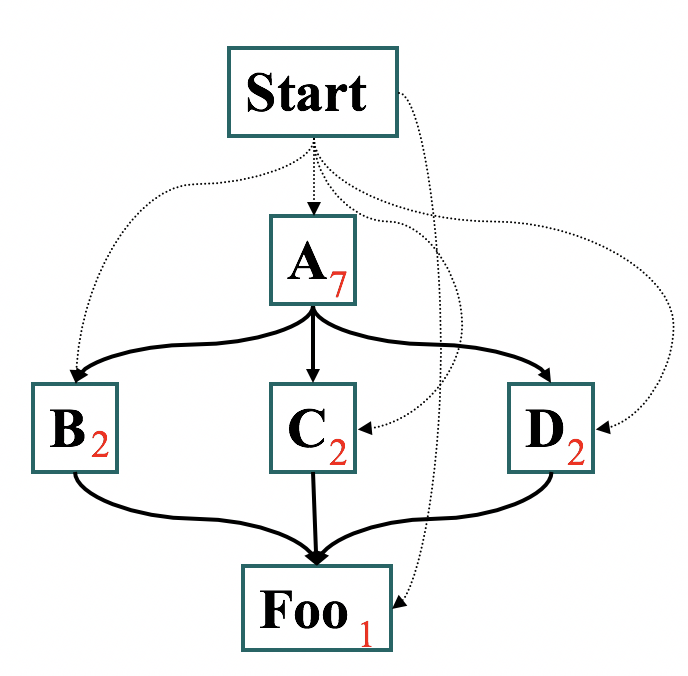
\includegraphics[width=0.4\textwidth]{images/callpaths.png}
\end{center}

\end{frame}



\begin{frame}
\frametitle{Another Call Graph}


Consider another diagram showing the relationships between functions, in which the numbers on the edges represent the number of invocations:

\begin{center}
	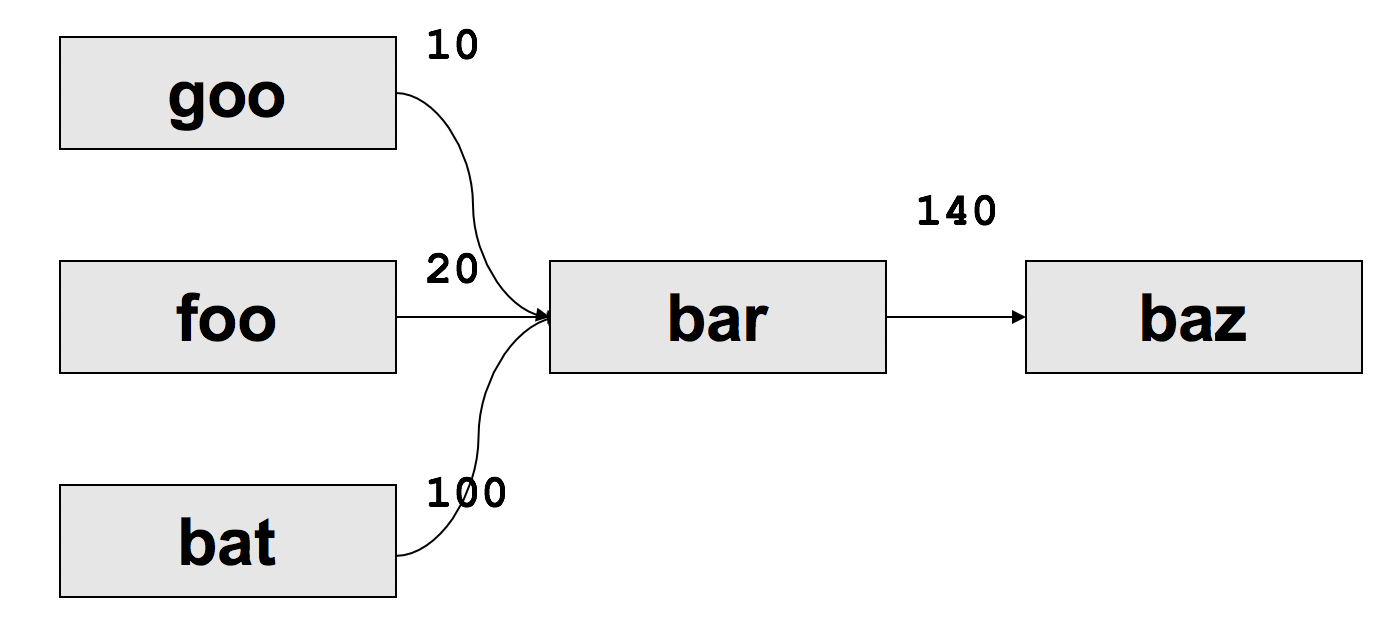
\includegraphics[width=\textwidth]{images/callpaths2.png}
\end{center}

\end{frame}



\begin{frame}
\frametitle{The POGO View of the World}

When considering what to do here, POGO takes the view like this:

\begin{center}
	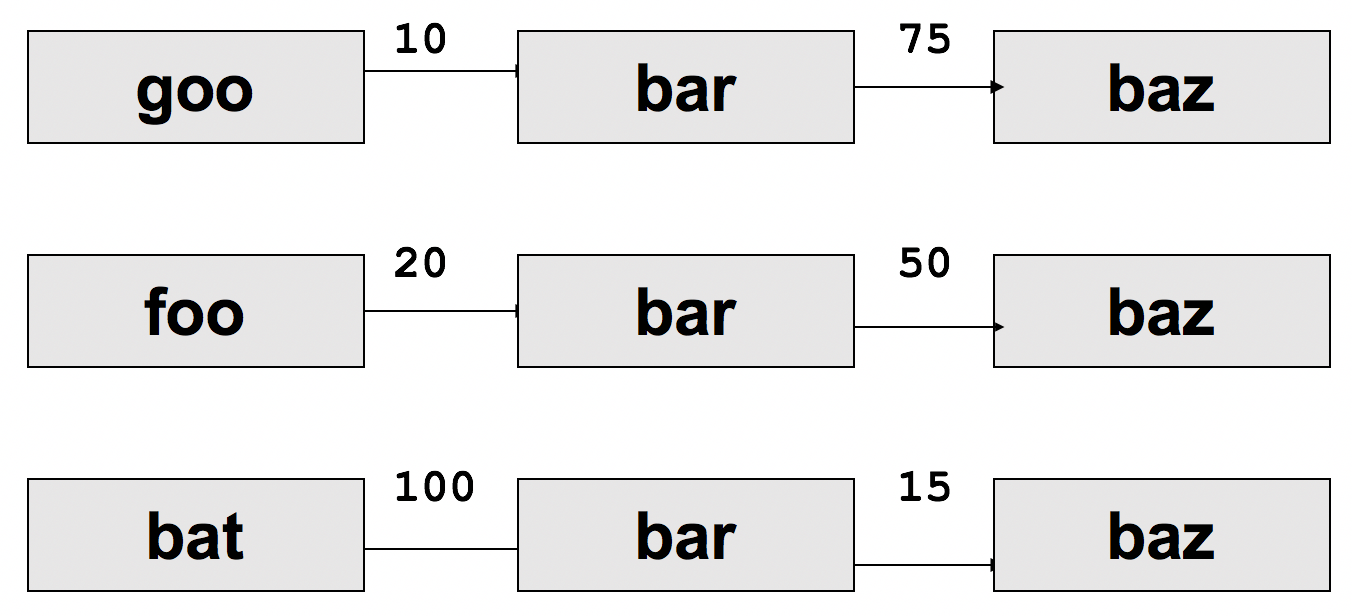
\includegraphics[width=\textwidth]{images/callpaths3.png}
\end{center}

\end{frame}



\begin{frame}
\frametitle{The POGO View of the World}

\begin{center}
	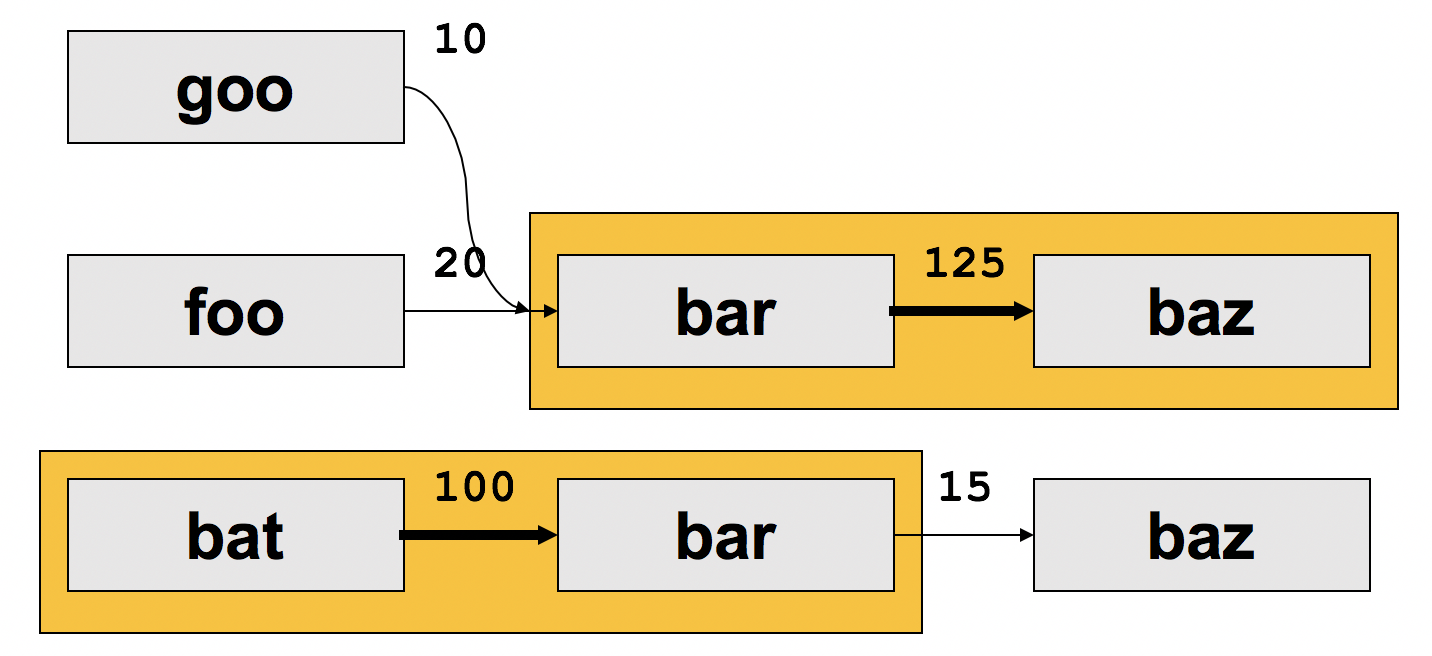
\includegraphics[width=\textwidth]{images/callpaths4.png}
\end{center}

\end{frame}




\begin{frame}
\frametitle{Page Locality}

Packing the blocks is also done based on this call graph profiling. 

The most common cases will be put next to each other, and, where possible, subsequent steps are put next to each other. 

The more we can pack related code together, the fewer page faults we get by jumping to some other section, causing a cache miss... 

If the function being called is in the same page as the call, it has achieved ``page locality''.

\end{frame}



\begin{frame}
\frametitle{Block Layout}

\begin{center}
	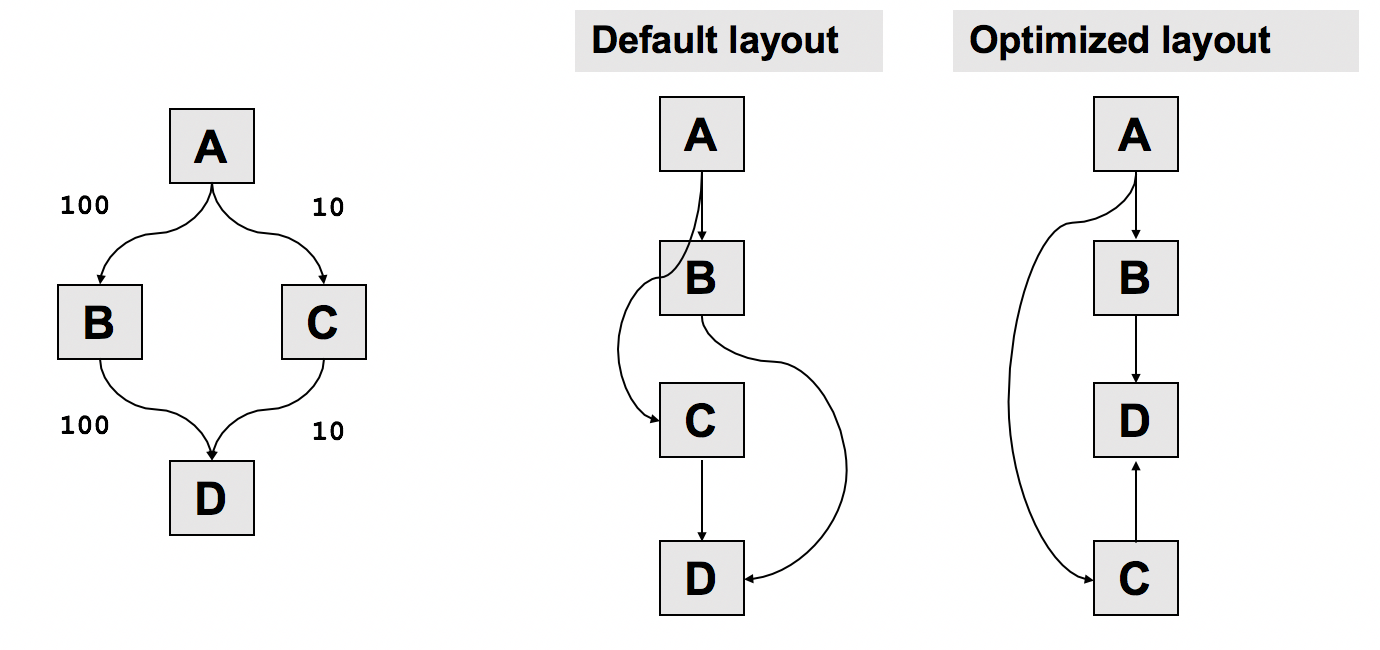
\includegraphics[width=\textwidth]{images/blocklayout.png}
\end{center}

\end{frame}



\begin{frame}
\frametitle{Dead Code?}

According to the author, the ``dead'' code goes in its own special block. 

I don't think they actually mean truly dead code, the kind that is compile-time determined to be unreachable. 

Instead they mean code that never gets invoked in any of the training runs.

But how well does it work?

\end{frame}



\begin{frame}
\frametitle{Benchmark Results}

The application under test is a standard benchmark suite (Spec2K):

\begin{center}
\begin{tabular}{l|l|l|l|l|l}
	\textbf{Spec2k:} & \textbf{sjeng} & \textbf{gobmk} & \textbf{perl} & \textbf{povray} & \textbf{gcc}\\ \hline
	\textbf{App Size:} &  {Small} & {Medium} & {Medium} & {Medium} & {Large} \\ \hline
	\textbf{Inlined Edge Count} & 50\% & 53\% & 25\% & 79\% & 65\% \\ \hline
	\textbf{Page Locality} & 97\% & 75\% & 85\% & 98\% & 80\% \\ \hline
	\textbf{Speed Gain} & 8.5\% & 6.6\% & 14.9\% & 36.9\% & 7.9\% \\ 
\end{tabular}
\end{center}

We can speculate about how well the results in a synthetic benchmark translate to real-world application performance...


\end{frame}

\end{document}

